\section{Dataset}
% motivation for creating this theme
\begin{frame}{Dataset}{}


    \begin{block}{}

        Training datasets of face images are needed as the SRCNN is a learning based super-resolution method.

        \begin{table}[]
            \resizebox{\textwidth}{!}{

                \begin{tabular}{|l|l|l|l|}
                    \hline
                    & \textbf{AR500}     & \textbf{AToF}       & \textbf{LFD}   \\ \hline
                    \textbf{Characteristics} & Similar conditions & Very large variation & Large variation \\ \hline
                    \textbf{Images}          & 500                & 153                 & 13300          \\ \hline
                \end{tabular}
            }
        \end{table}

        Several test datasets are also used (AR5, TDRF and SET5).
    \end{block}
\end{frame}


\begin{frame}{Dataset}{}
    \begin{block}{}
        \vspace{-1cm}
        \begin{columns}
            \begin{column}{0.1\textwidth}
                AR500\\
                ~\\
                ~\\
                ~\\
                AToF\\
                ~\\
                ~\\
                ~\\
                LFD
            \end{column}
            \hspace{-1cm}
            \begin{column}{1\textwidth}
                \begin{figure}[H]
                    \begin{subfigure}[b]{0.1\textwidth}
                        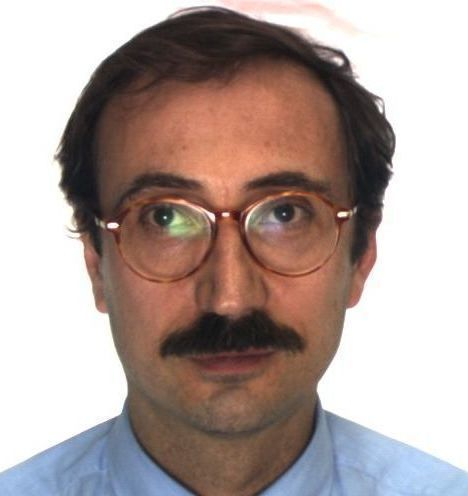
\includegraphics[width=\textwidth]{figs/ar1.jpg}
                    \end{subfigure}
                    \quad
                    \begin{subfigure}[b]{0.1\textwidth}
                        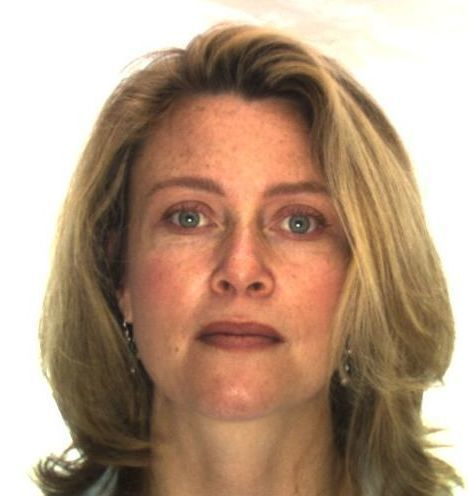
\includegraphics[width=\textwidth]{figs/ar2.jpg}
                    \end{subfigure}
                    \quad
                    \begin{subfigure}[b]{0.1\textwidth}
                        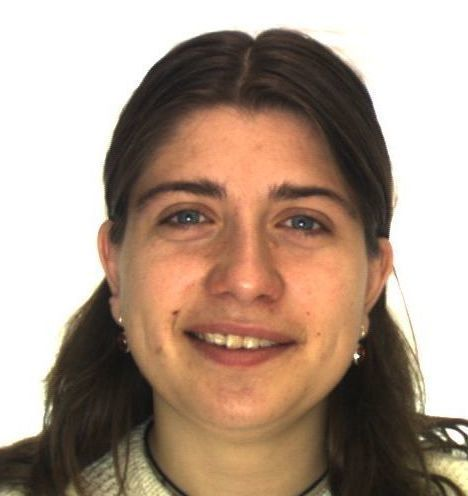
\includegraphics[width=\textwidth]{figs/ar3.jpg}
                    \end{subfigure}
                    \quad
                    \begin{subfigure}[b]{0.1\textwidth}
                        \includegraphics[width=\textwidth]{figs/ar4.jpg}
                    \end{subfigure}
                    \quad
                    \begin{subfigure}[b]{0.1\textwidth}
                        \includegraphics[width=\textwidth]{figs/ar5.jpg}
                    \end{subfigure}
                \end{figure}


                \begin{figure}[H]
                    \begin{subfigure}[b]{0.1\textwidth}
                        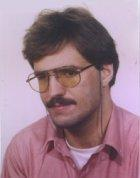
\includegraphics[width=\textwidth]{figs/atof1.jpg}
                    \end{subfigure}
                    \quad
                    \begin{subfigure}[b]{0.1\textwidth}
                        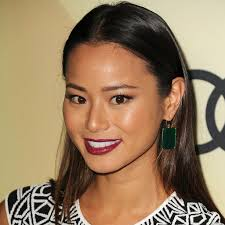
\includegraphics[width=\textwidth]{figs/atof2.jpg}
                    \end{subfigure}
                    \quad
                    \begin{subfigure}[b]{0.1\textwidth}
                        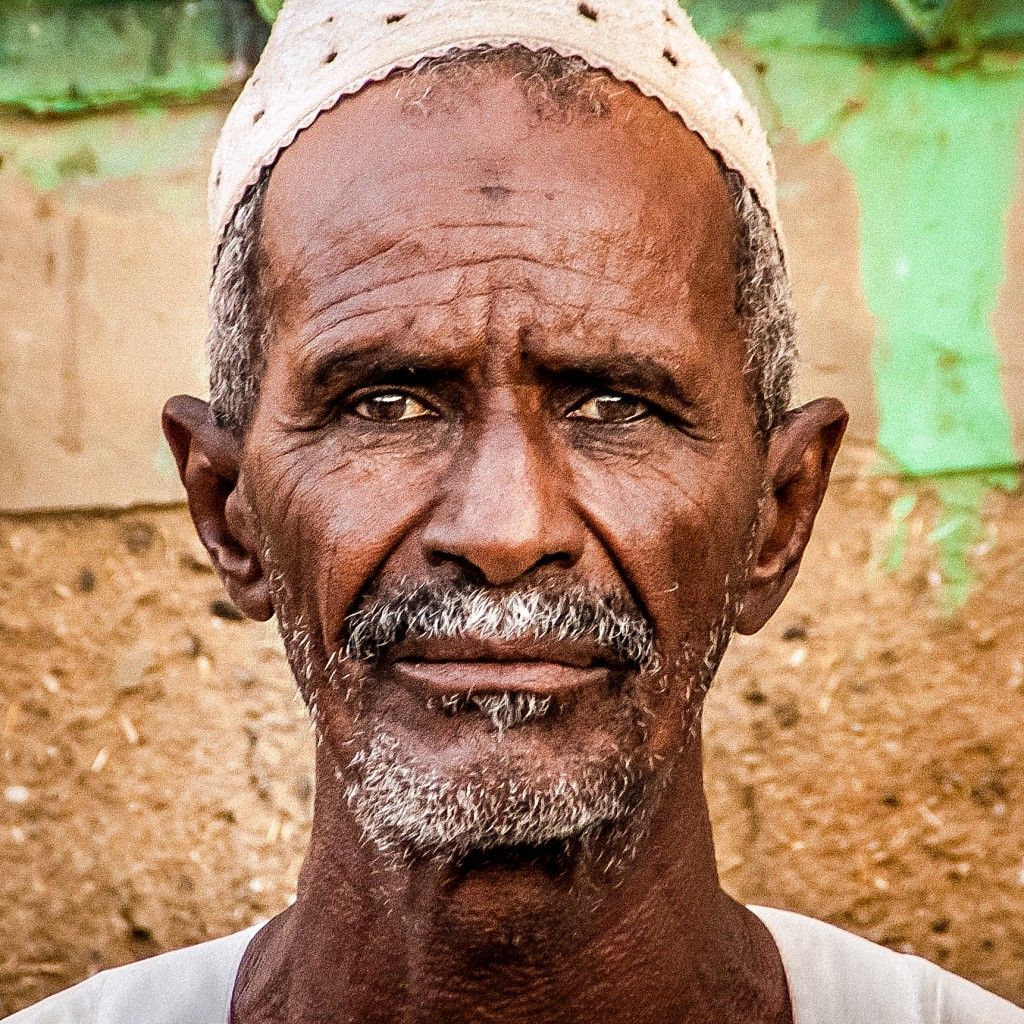
\includegraphics[width=\textwidth]{figs/atof3.jpg}
                    \end{subfigure}
                    \quad
                    \begin{subfigure}[b]{0.1\textwidth}
                        \includegraphics[width=\textwidth]{figs/atof4.jpg}
                    \end{subfigure}
                    \quad
                    \begin{subfigure}[b]{0.1\textwidth}
                        \includegraphics[width=\textwidth]{figs/atof5.jpg}
                    \end{subfigure}
                \end{figure}

                \begin{figure}[H]
                    \begin{subfigure}[b]{0.1\textwidth}
                        \includegraphics[width=\textwidth]{figs/lfd1.jpg}
                    \end{subfigure}
                    \quad
                    \begin{subfigure}[b]{0.1\textwidth}
                        \includegraphics[width=\textwidth]{figs/lfd2.jpg}
                    \end{subfigure}
                    \quad
                    \begin{subfigure}[b]{0.1\textwidth}
                        \includegraphics[width=\textwidth]{figs/lfd3.jpg}
                    \end{subfigure}
                    \quad
                    \begin{subfigure}[b]{0.1\textwidth}
                        \includegraphics[width=\textwidth]{figs/lfd4.jpg}
                    \end{subfigure}
                    \quad
                    \begin{subfigure}[b]{0.1\textwidth}
                        \includegraphics[width=\textwidth]{figs/lfd5.jpg}
                    \end{subfigure}
                \end{figure}


            \end{column}

        \end{columns}




    \end{block}
\end{frame}


